%%% Fiktivní kapitola s ukázkami sazby

\chapter{Vue.js framework}
Klientská část aplikace je postavena nad Vue.js frameworkem, jež je populární JavaScriptový framework na stavbu uživatelských rozhraní. Protože některé z jeho funkcionalit byly použity v klíčových částech aplikace, je nutné čtenáře obeznámit alespoň se základním principem fungování frameworku.

\section{Vuex}
Vue.js framework, podobně jako konkurenční React\footnote{\url{https://reactjs.org/}} (Facebook) nebo Angular\footnote{\url{https://angularjs.org/}} (Google), využívají principu sledování stavu aplikace (jejich dat) pro automatickou změnu DOMu webové stránky. V praxi to znamená, že programátor může velice snadno napsat kód, který generuje uživatelské rozhraní na základě dat, která mohou být libovolně měněna bez nutnosti řešit problém, zda ke změně vůbec došlo a které části aplikace mají být o změně stavu informovány. Ve Vue tuto funkcionalitu zastává právě Vuex\footnote{\url{https://vuex.vuejs.org/}}, jež je možný používat samostatně.

Vuex drží stav aplikace jako jeden objekt (tedy slouží jako centrální úložiště dat pro celou aplikaci). Tento objekt se nazývá \textbf{store}. Změny ve storu mohou být sledovány Vuexem pro vykonání libovolných akcí, například překreslení textu na stránce, jež byl vykreslen Vue frameworkem.

\newcommand{\inlinecode}{\texttt}

Vrátíme-li se k původnímu příkladu, programátorovi stačí přiřadit do proměnné, jež je spravovaná Vuexem, novou hodnotu a Vuex se postará o zavolání všech komponent, které tuto proměnnou využívají a tyto komponenty na stránce překreslí původní hodnotu na novou. Překreslení přitom proběhne až poté, co skončí průběh aktuální funkce. Tohoto je docíleno pomocí \\ \texttt{Window.requestAnimationFrame()}. Díky tomuto můžeme stav v rámci průběhu jedné funkce modifikovat vícekrát se skoro nulovým dopadem na celkový výkon aplikace.

\subsection{Computed properties}

Kromě této funkcionality Vuex nabízí takzvané \textbf{gettery}, jež jsou ve Vue frameworku nazývány jako \textbf{computed properties}. Jedná se o funkce, které využívají data ze storu pro výpočet dat nových. Výhoda takovýchto getterů je ta, že Vuex dokáže výsledky těchto funkcí cachovat a přepočítává je pouze tehdy, změní-li se data původní. Interně gettery fungují tak, že při zavolání klientské funkce Vuex sleduje které části storu byly dotázany a ty pak sleduje na změnu jež invaliduje cache konkrétního getteru. Při příštím požadavku na hodnotu se pak klientská funkce volá znovu a celá operace se opakuje.

Tyto computed properties jsou v aplikaci využívány často. Kupříkladu funkce, která počítá, zda je sousední uzel vybrán. Na takovouto hodnotu se v aplikaci mohu ptát libovolně krát, ale počítá se pouze tehdy, když se množina sousedních uzlů vrcholu změní, nebo se změní právě označení uzlu z množiny.

\subsection{Watchers}

Ve Vue lze využívat i \textbf{watch}ery, které umožňují registraci callbacku na změnu určité proměnné ve stavu. Watchery má smysl využívat tam, kde již data přestávají být spravována Vue frameworkem, tedy u knihoven třetích stran. Watchery, podobně jako překreslení komponent, jsou volány až po skončení probíhající funkce.

\subsection{Změna stavu}

Jak již bylo zmíněno, stav lze měnit přiřazením do proměnné, popřípadě voláním metod jako \texttt{.push()} na poli. Vuex dokáže tyto změny sledovat nahrazením původní proměnné (máme na mysli položku objektu) JavaScriptovým setterem. U polí dojde k obalení metody \texttt{.push()} jež registruje změnu stavu.

Tento přístup má několik nevýhod, které se promítly i při vývoji klientské aplikace:
\begin{itemize}
  \item Vue není plně kompatibilní s novými \textbf{ES6 kontejnery} \texttt{Map} a \texttt{Set} a proto jsou v aplikaci používány jen v rámci lokálních proměnných a mapa je nahrazena klasickým objektem.
  \item Protože je v JavaScriptu nemožné sledovat \textbf{vytvoření nové property objektu}, musí programátor v tomto případě volat ručně \texttt{Vue.set(target, propertyName/index, value)} a \texttt{Vue.delete}, popřípadě vytvořit nový objekt který nahradí ten původní.
  \item Je důležité mít na paměti, že data ve storu již nejsou původními objekty v pravém slova smyslu, ale veškeré fieldy a metody u polí byly nahrazeny, jak je zmíněno výše. Proto předání objektů a polí ze storu knihovnám třetích stran je nutné ošetřit \textbf{oklonováním objektu}, jinak může dojít k zaseknutí aplikace.
  \item Instance tříd \textbf{knihoven třetích stran může zaseknout aplikaci}, pokud ji uložíme do storu. Bohužel, tohoto je velmi snadné ve Vue frameworku dosáhnout omylem. Problém je rozebrán v následující kapitole.
\end{itemize}

\section{Vue framework}
Vue framework využívá takzvané komponenty. Komponentou se rozumí prvek na stránce se kterým má smysl pracovat samostatně. Každá komponenta má vlastní HTML, CSS a JS. Komponenty se mohou do sebe zanořovat a vytvářet tak větší komponenty z menších. Příkladem může být komponenta \textit{seznam} jež dokáže na stránku vykreslit senznam prvků. Takováto komponenta by pak mohla mít podkomponenty jako \textit{prvek seznamu}.

Každé komponentě lze předat data formou \textbf{properties} přičemž komponenta na základě těchto dat může vyrobit pod sebou další komponenty a předat jim část dat, která dostala.

Tyto předávána data jsou právě data ze storu. Vue framework doporučuje, aby data co koponenta dostane formou properties neupravovala přímo, ale místo toho posílala události rodičovské komponentě, která data upraví. Ve své práci jsem se \textbf{rozhodl toto doporučení ignorovat}, neboť by tímto vzrostla náročnočnost na správu aplikace.

\begin{figure}[h]
    \centering
    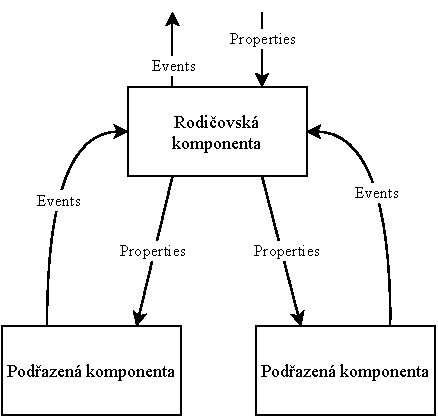
\includegraphics[width=0.5\textwidth]{media/vue.pdf}
    \caption{Doporučený způsob komunikace mezi komponentami ve Vue frameworku}
\end{figure}

\section{Loaders}
Kód Vue komponent se zapisuje do souborů s příponou \texttt{.vue}. Při sestavování aplikace se pak použije \texttt{vue-loader} který ze souboru vyextrahuje zvlášť CSS, JS a HTML a ty předá dál na zpracování. HTML kód komponent není ve skutečnosti pravý HTML. Jedná se nadstavbu umožňující psát speciální značky, jež rozhodují kolikrát a jestli vůbec se tag na stránce vyrenderuje. Tato HTML nadstavba je pak předána \texttt{vue-template-compiler} který vyrobí optimalizovaný JS kód jež renderuje HTML na základě stavu komponenty.

\newpage

\begin{prikl}
Ukázka jednoduché Vue komponenty \texttt{IndexedList} která má parametr \texttt{list} očekávající pole stringů. Tato komponenta vypíše pole v odrážkovém seznamu ve formě \texttt{index: hodnota}. Komponenta se sama stará o překreslení DOMu, když se změní data. Komponentu můžeme v jiné komponentě použít vložením \texttt{<indexed-list :list="inputData" />} kde \texttt{inputData} je proměnná obsahující pole stringů.

\begin{code}
<template>
  <ul>
    <li v-for="(item, index) in list" :key="index">
      {{index}}: {{ item }}
    </li>
  </ul>
</template>

<script lang="ts">
  import {Component, Prop} from "vue-property-decorator";
  import Vue from "vue";
  @Component
  export default class IndexedList extends Vue {
    @Prop() private list: string[];
  }
</script>

<style scoped>
  ul {
    color: red;
  }
</style>
\end{code}
\end{prikl}